% 图 71.2 —— 由 `checks/emit_hand.py` 自动拼出（probe 精测 + prims2 图元分解）
%%
% ⚠ 这是**稿子不是成品**：跑 `checks/checkhand.py 71.2` 看指标 + 看叠合图。
%%
%% ⚠ 待核：
%   · 本图 probe 报出阴影族 1 个 —— **本脚本不生成阴影**（要照原书手写）；prims2 的 strokes 里可能含阴影线，核对时留意别画重
%   · 可疑字形 1 项（空心圈 ⊙ 常被认成字母 o）—— 见文件末
%%
\documentclass[12pt]{standalone}
\usepackage{fontspec}
\setsansfont{Arial}
\newfontfamily\mfallback{DejaVu Sans}
\usepackage{tikz}
\begin{document}
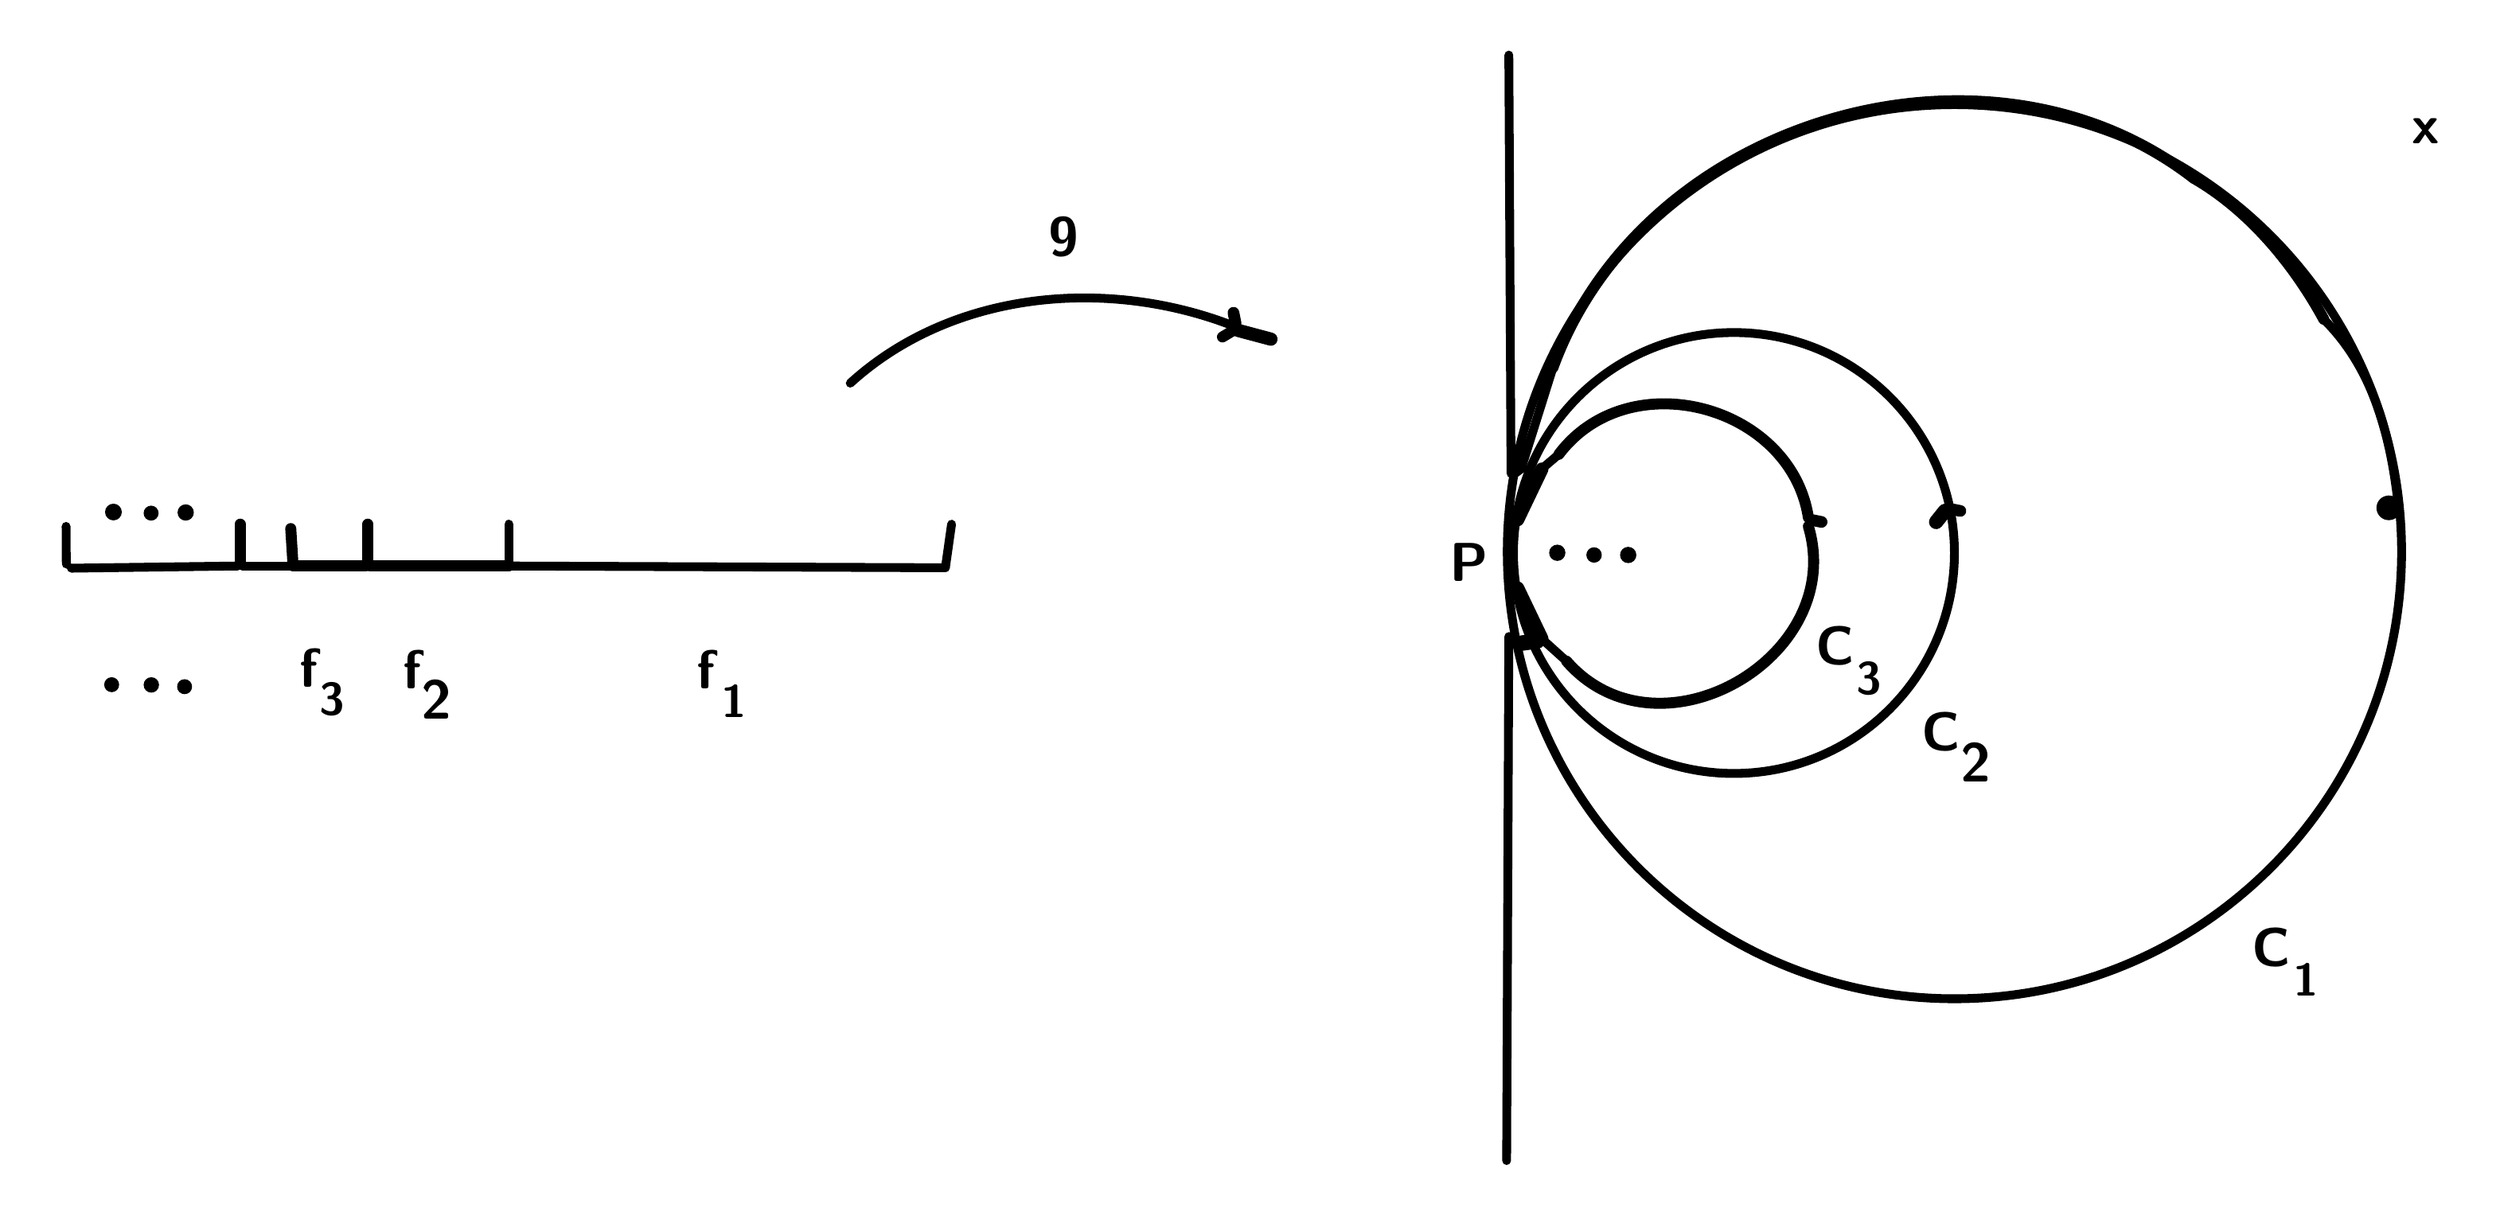
\begin{tikzpicture}[x=1pt, y=-1pt, line width=4.0pt, line cap=round, line join=round]

  %% ════ 填充区（prims2 的 fills）════

  %% ════ 直线段（prims2 的 strokes）════
  \draw[line width=4.0pt] (20.0,229.0) -- (20.1,246.1);
  \draw[line width=3.0pt] (20.1,246.1) -- (22.4,248.0);
  \draw[line width=4.0pt] (22.4,248.0) -- (98.0,247.0);
  \draw[line width=5.0pt] (122.0,230.0) -- (123.0,246.0);
  \draw[line width=6.0pt] (690.0,280.0) -- (679.0,257.0);
  \draw[line width=5.0pt] (156.0,247.0) -- (123.0,247.0);
  \draw[line width=5.0pt] (157.0,246.0) -- (157.0,228.0);
  \draw[line width=7.0pt] (688.0,281.0) -- (681.0,282.0);
  \draw[line width=4.0pt] (122.0,247.0) -- (100.0,247.0);
  \draw[line width=4.0pt] (695.0,157.0) -- (680.8,202.2);
  \draw[line width=4.9pt] (680.8,202.2) -- (677.0,205.0);
  \draw[line width=4.0pt] (697.7,196.3) -- (691.0,202.0);
  \draw[line width=5.3pt] (817.0,227.0) -- (812.0,226.0);
  \draw[line width=5.0pt] (550.0,140.0) -- (545.0,143.0);
  \draw[line width=5.3pt] (880.0,222.0) -- (875.0,221.0);
  \draw[line width=5.3pt] (550.0,132.0) -- (551.0,137.0);
  \draw[line width=6.5pt] (873.0,222.0) -- (869.0,227.0);
  \draw[line width=5.0pt] (158.0,247.0) -- (221.0,247.0);
  \draw[line width=4.0pt] (674.0,517.0) -- (675.0,279.0);
  \draw[line width=6.0pt] (552.0,140.0) -- (567.0,144.0);
  \draw[line width=6.0pt] (690.0,203.0) -- (679.0,226.0);
  \draw[line width=4.0pt] (691.0,281.0) -- (701.2,290.2);
  \draw[line width=5.0pt] (99.0,246.0) -- (99.0,228.0);
  \draw[line width=4.0pt] (221.0,228.0) -- (221.0,247.0);
  \draw[line width=4.0pt] (422.0,228.0) -- (419.2,247.8);
  \draw[line width=4.0pt] (419.2,247.8) -- (221.0,247.0);
  \draw[line width=4.0pt] (676.0,205.0) -- (675.0,15.0);

  %% ════ 曲线（prims2 的 curves —— 三段式，坐标同为 (y,x)）════
  \draw[line width=4.0pt] (1079.0,221.0) .. controls (1075.6,189.8) and (1068.3,158.1) .. (1045.0,135.0);
  \draw[line width=5.0pt] (1045.0,135.0) .. controls (1031.4,110.0) and (1011.2,85.5) .. (985.9,70.9);
  \draw[line width=5.0pt] (985.9,70.9) .. controls (891.4,-2.2) and (735.7,44.6) .. (695.0,157.0);
  \draw[line width=5.0pt] (811.0,225.0) .. controls (803.1,173.9) and (729.5,154.1) .. (697.7,196.3);
  \draw[line width=4.0pt] (550.0,138.0) .. controls (493.0,115.7) and (422.4,121.7) .. (376.0,164.0);
  \draw[line width=5.0pt] (701.2,290.2) .. controls (742.8,337.9) and (828.7,288.5) .. (811.0,229.0);

  %% ════ 圆 / 椭圆（probe 精测）════
  \draw (877.3,240.5) circle (203.0);
  \draw (777.2,241.1) circle (100.1);

  %% ════ 实心点 ════
  \fill (41.5,222.5) circle (3.8);
  \fill (58.6,223.0) circle (3.4);
  \fill (74.3,222.7) circle (3.7);
  \fill (697.0,241.0) circle (3.7);
  \fill (713.7,242.0) circle (3.5);
  \fill (729.2,242.0) circle (3.7);
  \fill (40.7,300.9) circle (3.4);
  \fill (58.7,301.0) circle (3.5);
  \fill (73.8,301.8) circle (3.4);
  \fill (1074.5,220.6) circle (5.6);

  %% ════ 标签（probe 直接给的 \node 行）════
  %% ⚠ 全部补了 fill=white：文字在最上层，否则与曲线交叉干扰
     \node[anchor=center,inner sep=0pt,fill=white,font=\fontsize{37.2}{46.5}\selectfont] at (1091.2,49.5) {\textsf{\textbf{\textit{x}}}};   % box(1080,36,20,22)
     \node[anchor=center,inner sep=0pt,fill=white,font=\fontsize{34.8}{43.5}\selectfont] at (473.0,97.4) {\textsf{\textbf{9}}};   % box(462,85,18,23)
     \node[anchor=center,inner sep=0pt,fill=white,font=\fontsize{29.8}{37.3}\selectfont] at (657.0,245.5) {\textsf{\textbf{\textit{P}}}};   % box(646,233,18,23)
     \node[anchor=center,inner sep=0pt,fill=white,font=\fontsize{32.9}{41.2}\selectfont] at (823.3,283.3) {\textsf{\textbf{\textit{C}}}};   % box(812,271,21,24)
     \node[anchor=center,inner sep=0pt,fill=white,font=\fontsize{28.5}{35.6}\selectfont] at (131.0,293.5) {\textsf{\textbf{\textit{f}}}};   % box(125,282,11,22)
     \node[anchor=center,inner sep=0pt,fill=white,font=\fontsize{29.1}{36.4}\selectfont] at (178.0,294.0) {\textsf{\textbf{\textit{f}}}};   % box(172,282,11,23)
     \node[anchor=center,inner sep=0pt,fill=white,font=\fontsize{27.8}{34.7}\selectfont] at (311.5,294.0) {\textsf{\textbf{\textit{f}}}};   % box(306,282,10,23)
     \node[anchor=center,inner sep=0pt,fill=white,font=\fontsize{21.9}{27.4}\selectfont] at (838.4,298.0) {\textsf{\textbf{3}}};   % box(833,289,10,17)
     \node[anchor=center,inner sep=0pt,fill=white,font=\fontsize{22.3}{27.9}\selectfont] at (140.9,307.6) {\textsf{\textbf{3}}};   % box(135,299,11,16)
     \node[anchor=center,inner sep=0pt,fill=white,font=\fontsize{23.6}{29.6}\selectfont] at (188.1,307.9) {\textsf{\textbf{2}}};   % box(182,299,11,17)
     \node[anchor=center,inner sep=0pt,fill=white,font=\fontsize{22.2}{27.8}\selectfont] at (323.1,308.4) {\textsf{\textbf{1}}};   % box(317,300,7,16)
     \node[anchor=center,inner sep=0pt,fill=white,font=\fontsize{32.9}{41.2}\selectfont] at (871.3,322.3) {\textsf{\textbf{\textit{C}}}};   % box(860,310,21,24)
     \node[anchor=center,inner sep=0pt,fill=white,font=\fontsize{22.9}{28.7}\selectfont] at (887.1,336.4) {\textsf{\textbf{2}}};   % box(881,328,11,16)
     \node[anchor=center,inner sep=0pt,fill=white,font=\fontsize{32.9}{41.2}\selectfont] at (1021.3,420.3) {\textsf{\textbf{\textit{C}}}};   % box(1010,408,21,24)
     \node[anchor=center,inner sep=0pt,fill=white,font=\fontsize{21.5}{26.9}\selectfont] at (1037.0,434.9) {\textsf{\textbf{1}}};   % box(1031,427,7,15)

  % 钉死画布：否则超出的图元/控制点会把页面撑大，1:1 回比就失准
  \pgfresetboundingbox
  \path[use as bounding box] (0,0) rectangle (1115,530);
\end{tikzpicture}
\end{document}

% ⚠ 待核清单（probe 拿不准，人眼过一遍）：
%   · 未识别/跳过：⑤ 跳过/未识别的字形
